\documentclass[11pt,twoside,a4paper]{article}
% http://www-h.eng.cam.ac.uk/help/tpl/textprocessing/latex_maths+pix/node6.html symboles de math
% http://fr.wikibooks.org/wiki/Programmation_LaTeX Programmation latex (wikibook)
%=========================== En-Tete =================================
%--- Insertion de paquetages (optionnel) ---
\usepackage[french]{babel}   % pour dire que le texte est en fran{\'e}ais
\usepackage{a4}	             % pour la taille   
\usepackage[T1]{fontenc}     % pour les font postscript
\usepackage{epsfig}          % pour gerer les images
%\usepackage{psfig}
\usepackage{amsmath, amsthm} % tres bon mode mathematique
\usepackage{amsfonts,amssymb}% permet la definition des ensembles
\usepackage{float}           % pour le placement des figure
\usepackage{verbatim}

\usepackage{multicol} % multicolonnes

\usepackage{longtable} % pour les tableaux de plusieurs pages

\usepackage[table]{xcolor} % couleur de fond des cellules de tableaux

\usepackage{lastpage}

\usepackage{multirow}

\usepackage{multicol} % pour {\'e}crire dans certaines zones en colonnes : \begin{multicols}{nb colonnes}...\end{multicols} 

% \usepackage[top=1.5cm, bottom=1.5cm, left=1.5cm, right=1.5cm]{geometry}
% gauche, haut, droite, bas, entete, ente2txt, pied, txt2pied
\usepackage{vmargin}
\setmarginsrb{0.20cm}{0.20cm}{0.20cm}{0.20cm}{15pt}{3pt}{42pt}{15pt}

\usepackage{lscape} % changement orientation page
%\usepackage{frbib} % enlever pour obtenir references en anglais
% --- style de page (pour les en-tete) ---
\pagestyle{empty}

% mettre du texte en diagonale sur le fond : tikz
\usepackage{tikz} 
\def\confidentialTIKZ{%
	\begin{tikzpicture}[remember picture,overlay]
	\node[rotate=60,scale=15,text opacity=0.1] at (current page.center) {Confidentiel};
	\end{tikzpicture}
}%

\def\TIKZcyberpunk2020{%
	\begin{tikzpicture}[remember picture,overlay]
	\node[rotate=60,scale=10,text opacity=0.1] at (current page.center) {Cyberpunk 2020};
	\end{tikzpicture}
}%

\def\txtTITLE{Feuille de personnage Cyberpunk 2020} %%%%% !! TITRE !! %%%%%
\def\imgCORNER{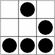
\includegraphics[width=0.25cm]{../../../../../imgGraphics/logos/glider/logo-glider.png}}

\def\imgGLIDERLEFTT{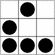
\includegraphics[width=1.95cm]{../../../../../imgGraphics/logos/glider/logo-glider-left.png}}
\def\imgGLIDERRIGHT{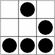
\includegraphics[width=1.95cm]{../../../../../imgGraphics/logos/glider/logo-glider-right.png}}

\def\imgGLIDERLEFTTsmall{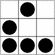
\includegraphics[width=0.25cm]{../../../../../imgGraphics/logos/glider/logo-glider-left.png}}
\def\imgGLIDERRIGHTsmall{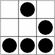
\includegraphics[width=0.25cm]{../../../../../imgGraphics/logos/glider/logo-glider-right.png}}

% % % en-tete et pieds de page configurables : fancyhdr.sty

% http://www.trustonme.net/didactels/250.html

% http://ww3.ac-poitiers.fr/math/tex/pratique/entete/entete.htm
% http://www.ctan.org/tex-archive/macros/latex/contrib/fancyhdr/fancyhdr.pdf
\usepackage{fancyhdr}
\pagestyle{fancy}
	% \renewcommand{\chaptermark}[1]{\markboth{#1}{}}
	% \renewcommand{\sectionmark}[1]{\markright{\thesection\ #1}}
\fancyhf{}
\fancyhead[LE,RO]{\bfseries\thepage \TIKZcyberpunk2020 }
\fancyhead[LO]{\bfseries\rightmark}
\fancyhead[RE]{\bfseries\leftmark}
\fancyfoot[LE]{\thepage /\pageref{LastPage} \hfill
	\scriptsize{\txtTITLE} % TITLE
\hfill \imgGLIDERLEFTTsmall }
\fancyfoot[RO]{\imgGLIDERRIGHTsmall \hfill
	\scriptsize{\txtTITLE} % TITLE
\hfill \thepage /\pageref{LastPage}}
\renewcommand{\headrulewidth}{0.5pt}
\renewcommand{\footrulewidth}{0.5pt}
\addtolength{\headheight}{0.5pt}
% \fancypagestyle{plain}{
	% \fancyhead{}
	% \renewcommand{\headrulewidth}{0pt}
% }

\def\smallbox{%
	\setlength{\unitlength}{0.5cm}
	\fbox{
		\begin{picture}(1, 1)(0,0)
		\end{picture}
	}
}%

%%%%%%%%%%% SOME VALUES IN ENGLISH %%%%%%%%%%%%%%%%%%%%%
\def\ENdefNom{\textbf{Name} \dotfill }


%%%%%%%%%%% QUELQUES VALEURS EN FRANCAIS %%%%%%%%%%%%%%%%%%%%%
\def\FRdefNom{\small \textbf{Nom} \dotfill }
\def\FRdefRole{\small \textbf{R{\^o}le} \dotfill }
\def\FRdefPPerso{\small \textbf{Points de \newline Personnage} \dotfill }
\def\FRdefCaract{\small \textbf{Caract{\'e}ristiques} \dotfill }
\def\FRdefLocali{\small \textbf{Localisation \newline Armure PA} \dotfill }
\def\FRdefSauveg{\small \textbf{Sauvegarde} \hrulefill \dotfill }
\def\FRdefMCMCMC{\small \textbf{MC} \hrulefill \dotfill }
\def\FRdefBonusD{\small \textbf{Bonus Domages} \hrulefill \dotfill }
\def\FRdefCOMPET{\small \textbf{Comp{\'e}tences} \dotfill }

%%%%% exchange (find & replace) between 'ENdef' end 'FRdef' from here to forward (43 occurences) %%%%%

\def\CELblackTXTWhite{\cellcolor{black} \color{white}}


%============================= Corps =================================
\begin{document}

\setlength\parindent{0pt}

\small

\begin{tabular}{ p{0.47\textwidth} p{0.50\textwidth} } 
	\begin{tabular}{ p{0.47\textwidth} }
		CyberPunk 2020 --- Fiche de personnage \\
		
\includegraphics[width=5.00cm]{../../../../../imgGraphics/rolePlayingGame/cyberpunk2020logo.jpg} \\
		\fbox{ \begin{minipage}[ht]{0.45\textwidth} 
			\textsc{Dessin du Personnage} 
			\newline \newline \newline \newline \newline 
			\newline \newline \newline \newline \newline 
			\newline \newline \newline \newline \newline
			\newline \newline \newline \newline \newline
		\end{minipage} } \\ 
		%% 
\includegraphics[width=5.00cm]{../../../../../imgGraphics/rolePlayingGame/cyberpunk2020logo.jpg} \\
	\end{tabular}
	&	
	\begin{tabular}[c]{ p{0.15\textwidth} p{5.00cm} } %% p{0.60\textwidth}}
		\CELblackTXTWhite \FRdefNom		& \fbox{ \begin{minipage}[ht]{4.80cm} \dotfill \newline \dotfill \newline \end{minipage} }	 \\
										&														 \\
		\CELblackTXTWhite \FRdefRole	& 
			\footnotesize %%%%%
			\begin{tabular}[c]{ p{0.10\textwidth} p{0.10\textwidth} }
				\fbox{ } Solo		&	\fbox{ } Rocker		 \\
				\fbox{ } NetRunner	&	\fbox{ } Media		 \\
				\fbox{ } Fixer		&	\fbox{ } Cop		 \\
				\fbox{ } Corpo		&	\fbox{ } Techie		 \\
				\fbox{ } MedTechie	&	\fbox{ } Nomade		 \\
			\end{tabular} \\
										&														 \\
		\CELblackTXTWhite \FRdefPPerso 	& 
			\fbox{ \begin{minipage}[ht]{4.80cm} \dotfill \newline \end{minipage} }
			R{\'e}putation	\hrulefill \dotfill \newline
			PC Acquis		\hrulefill \dotfill \newline
			Humanit{\'e}	\hrulefill \dotfill %% \newline
			\\
										&														 \\
		\CELblackTXTWhite \FRdefCaract 	& 
			\footnotesize %%%%%
			\begin{tabular}[c]{|c|c|c|c|}
				\hline
				INT		&			&	REF			&	/		\\
				\hline
				TECH	&			&	SF			&			\\
				\hline
				BT		&			&	CH			&			\\
				\hline
				MV		&			&	CON			&			\\
				\hline
				EMP		&	/		&	Course		&			\\
				\hline
				Saut	&			&	Lev{\'e}e	&			\\
				\hline
			\end{tabular} \\
		 								&														 \\
		\CELblackTXTWhite \FRdefLocali	&
			{\scriptsize
			\begin{tabular}[c]{|c|c|c|}
				\hline
				T{\^e}te (1)	&	Bras D (5)		&	Jambe D	(7-8)	\\
				\hline
								&					&					\\
				\hline
				Torse (2-4)		&	Bras G (6)		&	Jambe G (9-10)	\\
				\hline
								&					&					\\
				\hline
			\end{tabular} } \\
	\end{tabular} 					\\
	\FRdefSauveg					& \FRdefMCMCMC						 \\
	\FRdefBonusD					& \CELblackTXTWhite \FRdefCOMPET	 \\
\end{tabular}

\scriptsize Ajoutez les points de comp{\'e}tence {\`a} la caract{\'e}ristique applicable, inscrivez le total dans la case. Inscrivez les comp{\'e}tences en puce par un X {\`a} c{\^o}t{\'e} de la case. ~\\ 

\begin{tabular}[c]{p{0.30\textwidth} p{0.30\textwidth} p{0.30\textwidth}}
	\textbf{\textsc{Capacit{\'e}s sp{\'e}ciales}}				&	\textbf{\textsc{REF} (R{\'e}flexes)}				&	\textbf{\textsc{TECH} (Technique)}	\\
	Autorit{\'e} (Cop)					\dotfill	\fbox{ }	&	Armes Automatiques			\dotfill	\fbox{ }	&	A{\'e}rotech				\dotfill	\fbox{ }	\\
	Com. Charismatique (Rocker)			\dotfill	\fbox{ }	&	Armes Lourdes				\dotfill	\fbox{ }	&	Armurier					\dotfill	\fbox{ }	\\
	Cr{\'e}dibilit{\'e} (Media)			\dotfill	\fbox{ }	&	Arts Martial 1	\hrulefill	\dotfill	\fbox{ }	&	AVtech						\dotfill	\fbox{ }	\\
	Famille (Nomade)					\dotfill	\fbox{ }	&	Arts Martial 2	\hrulefill	\dotfill	\fbox{ }	&	Concevoir cyberdeck			\dotfill	\fbox{ }	\\
	Indic (Fixer)						\dotfill	\fbox{ }	&	Arts Martial 3	\hrulefill	\dotfill	\fbox{ }	&	Contrefa\c{c}on				\dotfill	\fbox{ }	\\
	Interface (NetRunner)				\dotfill	\fbox{ }	&	Conduite Automobiles		\dotfill	\fbox{ }	&	Crocheter					\dotfill	\fbox{ }	\\
	Ressources (Corporate)				\dotfill	\fbox{ }	&	Conduite Engins Lourds		\dotfill	\fbox{ }	&	Cybertech					\dotfill	\fbox{ }	\\
	Sens du contact (Solo)				\dotfill	\fbox{ }	&	Danse						\dotfill	\fbox{ }	&	D{\'e}quisement				\dotfill	\fbox{ }	\\
	Syst{\`e}me D (Techie)				\dotfill	\fbox{ }	&	Discr{\'e}tion				\dotfill	\fbox{ }	&	{\'E}lectronique			\dotfill	\fbox{ }	\\
	Technique M{\'e}dicale (MedTech)	\dotfill	\fbox{ }	&	Escrime						\dotfill	\fbox{ }	&	Explosifs					\dotfill	\fbox{ }	\\
	\textbf{\textsc{BT} (Beaut{\'e})}							&	Esquive						\dotfill	\fbox{ }	&	Gentech						\dotfill	\fbox{ }	\\
	Habillement et Style				\dotfill	\fbox{ }	&	Fusil						\dotfill	\fbox{ }	&	Graphismes					\dotfill	\fbox{ }	\\
	Look								\dotfill	\fbox{ }	&	Lutte						\dotfill	\fbox{ }	&	Gyrotech					\dotfill	\fbox{ }	\\
	\textbf{\textsc{CON} (Constitution)}						&	M{\^e}l{\'e}e				\dotfill	\fbox{ }	&	Musique						\dotfill	\fbox{ }	\\
	Endurance							\dotfill	\fbox{ }	&	Moto						\dotfill	\fbox{ }	&	Pharmacologie				\dotfill	\fbox{ }	\\
	Force								\dotfill	\fbox{ }	&	Piloter avion				\dotfill	\fbox{ }	&	Photos et films				\dotfill	\fbox{ }	\\
	Natation							\dotfill	\fbox{ }	&	Piloter dirigeable			\dotfill	\fbox{ }	&	Pickpocket					\dotfill	\fbox{ }	\\
	\textbf{\textsc{EMP} (Empathie)}							&	Piloter gyro				\dotfill	\fbox{ }	&	Premiers soins				\dotfill	\fbox{ }	\\
	Baratin et Persuasion				\dotfill	\fbox{ }	&	Piloter h{\'e}licopt{\`e}re	\dotfill	\fbox{ }	&	S{\'e}curit{\'e} {\'e}lectronique		\dotfill	\fbox{ }	\\
	Commandement						\dotfill	\fbox{ }	&	Piloter jet					\dotfill	\fbox{ }	&	Utilisation caisson cryo	\dotfill	\fbox{ }	\\
	Interview							\dotfill	\fbox{ }	&	Pistolet					\dotfill	\fbox{ }	&								\dotfill	\fbox{ }	\\
	Perception humaine					\dotfill	\fbox{ }	&	Tir {\`a} l'arc				\dotfill	\fbox{ }	&								\dotfill	\fbox{ }	\\
	Performance							\dotfill	\fbox{ }	&	\textbf{\textsc{INT} (Intelligence)}				&														\\
	S{\'e}duction						\dotfill	\fbox{ }	&	Anthropologie				\dotfill	\fbox{ }	&	Histoire					\dotfill	\fbox{ }	\\
	Social								\dotfill	\fbox{ }	&	Biblioth{\`e}que			\dotfill	\fbox{ }	&	Investissement				\dotfill	\fbox{ }	\\
	\textbf{\textsc{MV} (Mouvement)}							&	Biologie					\dotfill	\fbox{ }	&	Jeu							\dotfill	\fbox{ }	\\
	Athl{\'e}tisme						\dotfill	\fbox{ }	&	Botanique					\dotfill	\fbox{ }	&	Math{\'e}matiques				\dotfill	\fbox{ }	\\
																&	Chimie						\dotfill	\fbox{ }	&	Perception					\dotfill	\fbox{ }	\\
	Langue				\hrulefill		\dotfill	\fbox{ }	&	Composition					\dotfill	\fbox{ }	&	Physique					\dotfill	\fbox{ }	\\
	Langue				\hrulefill		\dotfill	\fbox{ }	&	Connaissance du syst{\`e}me	\dotfill	\fbox{ }	&	Programmation				\dotfill	\fbox{ }	\\
	Langue				\hrulefill		\dotfill	\fbox{ }	&	Diagnostic					\dotfill	\fbox{ }	&	Se cacher / Semer			\dotfill	\fbox{ }	\\
	Expertise			\hrulefill		\dotfill	\fbox{ }	&	{\'E}ducation				\dotfill	\fbox{ }	&	Suivre / Pister				\dotfill	\fbox{ }	\\
	Expertise			\hrulefill		\dotfill	\fbox{ }	&	Enseignement				\dotfill	\fbox{ }	&	Survivre en milieu hostile	\dotfill	\fbox{ }	\\
	Expertise			\hrulefill		\dotfill	\fbox{ }	&	G{\'e}ologie				\dotfill	\fbox{ }	&	Zoologie					\dotfill	\fbox{ }	\\
																&	Gestion						\dotfill	\fbox{ }	&								\dotfill	\fbox{ }	\\
	\textbf{\textsc{SF} (Sang-Froid)}							&	\textbf{\textsc{Autres}}													&														\\
	Connaissance de la rue				\dotfill	\fbox{ }	&								\dotfill	\fbox{ }	&								\dotfill	\fbox{ }	\\
	{\'E}loquence						\dotfill	\fbox{ }	&								\dotfill	\fbox{ }	&								\dotfill	\fbox{ }	\\
	Interrogatoire						\dotfill	\fbox{ }	&								\dotfill	\fbox{ }	&								\dotfill	\fbox{ }	\\
	Intimidation						\dotfill	\fbox{ }	&								\dotfill	\fbox{ }	&								\dotfill	\fbox{ }	\\
	R{\'e}sister (Torture et Drogues)	\dotfill	\fbox{ }	&								\dotfill	\fbox{ }	&								\dotfill	\fbox{ }	\\
										\dotfill	\fbox{ }	&								\dotfill	\fbox{ }	&								\dotfill	\fbox{ }	\\
										\dotfill	\fbox{ }	&								\dotfill	\fbox{ }	&								\dotfill	\fbox{ }	\\
										
											
	
\end{tabular}

\clearpage

\begin{tabular}{|p{0.95\textwidth}|}
	\normalsize
	\CELblackTXTWhite \textsc{\textbf{\LARGE Vie et Contacts}}	\\
																\\
	\begin{tabular}{ p{0.40\textwidth} c p{0.45\textwidth} }
		\begin{tabular}{|p{8.00cm}|}
			\CELblackTXTWhite \textsc{\textbf{\Large {\'E}v{\`e}nements de la vie}} \\
			\begin{enumerate}
				\item[17] \hrulefill
				\item[18] \hrulefill
				\item[19] \hrulefill
				\item[20] \hrulefill
				\item[21] \hrulefill
				\item[22] \hrulefill
				\item[23] \hrulefill
				\item[24] \hrulefill
				\item[25] \hrulefill
				\item[26] \hrulefill
				\item[27] \hrulefill
				\item[28] \hrulefill
				\item[29] \hrulefill
				\item[30] \hrulefill
			\end{enumerate} \\
			\hline
		\end{tabular}	&	&	
		\begin{tabular}{|p{1.50cm}|p{7.00cm}|}
			\multicolumn{2}{|p{9.00cm}|}{\CELblackTXTWhite \textsc{\textbf{\Large Amis / Contacts}} }	\\
			Nom		&	R{\^o}le	\\	\hline
					&				\\	\hline
					&				\\	\hline
					&				\\	\hline
					&				\\	\hline
					&				\\	\hline
					&				\\	\hline
					&				\\	\hline
					&				\\	\hline
					&				\\	\hline
					&				\\	\hline
					&				\\	\hline
					&				\\	\hline
					&				\\	\hline
					&				\\	\hline
					&				\\	\hline
					&				\\	\hline
					&				\\	\hline
					&				\\	\hline
		\end{tabular}	\\
		
			&		&		\\
		
		\begin{tabular}{|p{8.00cm}|}
			\CELblackTXTWhite \textsc{\textbf{\Large Histoire Personnelle}} \\
			\begin{enumerate}
				\item[] 
				\item[]
				\item[]
				\item[]
				\item[]
				\item[]
				\item[]
				\item[]
				\item[]
				\item[]
			\end{enumerate} \\
			\hline
		\end{tabular}	\newline	\newline	\newline
		\begin{tabular}{|p{1.00cm}|p{6.60cm}|}
			\multicolumn{2}{|p{8.00cm}|}{\CELblackTXTWhite \textsc{\textbf{\Large R{\'e}sidence}} }	\\
			Adresse				&						\\	\hline
			Quartier			&						\\	\hline
			Loyer				&						\\	\hline
			N~\degres  Tel		&						\\	\hline
			S{\'e}curit{\'e}	&						\\	\hline
			Options				&						\\	\hline
		\end{tabular}	&	&	
		\begin{tabular}{|p{1.50cm}|p{7.00cm}|}
			\multicolumn{2}{|p{9.00cm}|}{\CELblackTXTWhite \textsc{\textbf{\Large Liste Noire (Ennemis)}} }	\\
			Nom		&	R{\^o}le / Cause	\\	\hline
					&						\\	\hline
					&						\\	\hline
					&						\\	\hline
					&						\\	\hline
					&						\\	\hline
					&						\\	\hline
					&						\\	\hline
					&						\\	\hline
					&						\\	\hline
					&						\\	\hline
					&						\\	\hline
					&						\\	\hline
					&						\\	\hline
					&						\\	\hline
					&						\\	\hline
		\end{tabular}	\newline	\newline	\newline
		\begin{tabular}{|p{2.70cm}|p{2.70cm}|p{2.70cm}|}
			\multicolumn{3}{|p{9.00cm}|}{\CELblackTXTWhite \textsc{\textbf{\Large Euros \$}} }	\\
			Carte		&	Poche	& Compte	\\	\hline
						&			& 			\\	\hline
		\end{tabular}	\\
		
			&		&		\\
		
		\begin{tabular}{|p{1.00cm}|p{6.60cm}|}
			\multicolumn{2}{|p{8.00cm}|}{\CELblackTXTWhite \textsc{\textbf{\Large Groupe (PJ)}} }	\\
			Nom		&	R{\^o}le			\\	\hline
					&						\\	\hline
					&						\\	\hline
					&						\\	\hline
					&						\\	\hline
					&						\\	\hline
					&						\\	\hline
					&						\\	\hline
					&						\\	\hline
					&						\\	\hline
					&						\\	\hline
					&						\\	\hline
					&						\\	\hline
					&						\\	\hline
					&						\\	\hline
					&						\\	\hline
		\end{tabular}	&	&	
		\begin{tabular}{|p{1.50cm}|p{6.60cm}|}
			\multicolumn{2}{|p{9.00cm}|}{\CELblackTXTWhite \textsc{\textbf{\Large Adresses}} }	\\
			Lieu	&	Description			\\	\hline
					&						\\	\hline
					&						\\	\hline
					&						\\	\hline
					&						\\	\hline
					&						\\	\hline
					&						\\	\hline
					&						\\	\hline
					&						\\	\hline
					&						\\	\hline
					&						\\	\hline
					&						\\	\hline
					&						\\	\hline
					&						\\	\hline
					&						\\	\hline
					&						\\	\hline
		\end{tabular}	\\
	\end{tabular} \\
	
			\\
	\hline
	
\end{tabular}

\clearpage

\begin{tabular}{|p{0.95\textwidth}|}
	\normalsize
	\CELblackTXTWhite \textsc{\textbf{\LARGE Armes, Cybern{\'e}tique et Mat{\'e}riels}}	\\
																						\\
	\begin{tabular}{ p{0.40\textwidth} p{0.030\textwidth} p{0.40\textwidth} }
		\begin{tabular}{|p{6.25cm}|p{0.50cm}|p{1.25cm}|}
			\multicolumn{3}{|p{8.85cm}|}{\CELblackTXTWhite \textsc{\textbf{\Large Cybern{\'e}tiques}} }	\\
			Type	&	PH	&	Co{\^u}t	\\	\hline
					&		&				\\	\hline
					&		&				\\	\hline
					&		&				\\	\hline
					&		&				\\	\hline
					&		&				\\	\hline
					&		&				\\	\hline
					&		&				\\	\hline
					&		&				\\	\hline
					&		&				\\	\hline
					&		&				\\	\hline
					&		&				\\	\hline
					&		&				\\	\hline
					&		&				\\	\hline
					&		&				\\	\hline
					&		&				\\	\hline
					&		&				\\	\hline
					&		&				\\	\hline
					&		&				\\	\hline
					&		&				\\	\hline
					&		&				\\	\hline
					&		&				\\	\hline
					&		&				\\	\hline
					&		&				\\	\hline
					&		&				\\	\hline
					&		&				\\	\hline
					&		&				\\	\hline
					&		&				\\	\hline
					&		&				\\	\hline
					&		&				\\	\hline
					&		&				\\	\hline
		\end{tabular} &		&	
		\begin{tabular}{|p{7.00cm}|p{1.50cm}|}
			\multicolumn{2}{|p{9.00cm}|}{\CELblackTXTWhite \textsc{\textbf{\Large Mat{\'e}riel}} }	\\
			Type	&	Co{\^u}t	\\	\hline
					&				\\	\hline
					&				\\	\hline
					&				\\	\hline
					&				\\	\hline
					&				\\	\hline
					&				\\	\hline
					&				\\	\hline
					&				\\	\hline
					&				\\	\hline
					&				\\	\hline
					&				\\	\hline
					&				\\	\hline
					&				\\	\hline
					&				\\	\hline
					&				\\	\hline
					&				\\	\hline
					&				\\	\hline
					&				\\	\hline
					&				\\	\hline
					&				\\	\hline
					&				\\	\hline
					&				\\	\hline
					&				\\	\hline
					&				\\	\hline
					&				\\	\hline
					&				\\	\hline
					&				\\	\hline
					&				\\	\hline
					&				\\	\hline
					&				\\	\hline
		\end{tabular} \\
	\end{tabular} \\
	\\ \\ \\
	
	\begin{tabular}{|p{3.00cm}|p{1.00cm}|p{2.00cm}|p{2.00cm}|p{2.00cm}|p{1.00cm}|p{1.00cm}|p{1.00cm}|p{1.00cm}|p{1.00cm}|p{2.00cm}|}
		\multicolumn{11}{|p{18.90cm}|}{\CELblackTXTWhite \textsc{\textbf{\Large Armes}} }	\\
		Nom	&	Type	&	Pr{\'e}cision	&	Dissimulation	&	Dommages	&	Chargeur	&	Restant	&	Tir	&	Fiabilit{\'e}	&	Port{\'e}e	\\	\hline
			&			&					&					&				&				&			&		&					&				\\	\hline
			&			&					&					&				&				&			&		&					&				\\	\hline
			&			&					&					&				&				&			&		&					&				\\	\hline
			&			&					&					&				&				&			&		&					&				\\	\hline
			&			&					&					&				&				&			&		&					&				\\	\hline
			&			&					&					&				&				&			&		&					&				\\	\hline
			&			&					&					&				&				&			&		&					&				\\	\hline
			&			&					&					&				&				&			&		&					&				\\	\hline
			&			&					&					&				&				&			&		&					&				\\	\hline
			&			&					&					&				&				&			&		&					&				\\	\hline
	\end{tabular}	\\	\\	\\
	
	\begin{tabular}{|p{4.00cm}|p{4.00cm}|p{0.25cm}|p{1.75cm}|p{1.00cm}|p{1.00cm}|p{1.00cm}|p{1.00cm}|p{1.00cm}|}
		\multicolumn{9}{|p{18.90cm}|}{\CELblackTXTWhite \textsc{\textbf{\Large V{\'e}hicule}} }	\\
		Nom : 				&	Options		&	\multicolumn{3}{|p{3.00cm}|}{Localisation d{\'e}g{\^a}ts}		&	
												\multicolumn{2}{|p{2.00cm}|}{Blindage}							&	
												\multicolumn{2}{|p{2.00cm}|}{D{\'e}g{\^a}ts}					\\	\hline
		Type : 				&				&	1	&	\multicolumn{2}{|p{2.75cm}|}{ }	&	\multicolumn{2}{|p{2.00cm}|}{ }		&	\multicolumn{2}{|p{2.00cm}|}{}	\\	\hline
		Vitesse : 			&				&	2	&	\multicolumn{2}{|p{2.75cm}|}{ }	&	\multicolumn{2}{|p{2.00cm}|}{ }		&	\multicolumn{2}{|p{2.00cm}|}{}	\\	\hline
		{\'E}quipage : 		&				&	3	&	\multicolumn{2}{|p{2.75cm}|}{ }	&	\multicolumn{2}{|p{2.00cm}|}{ }		&	\multicolumn{2}{|p{2.00cm}|}{}	\\	\hline
		Passagers : 		&				&	4	&	\multicolumn{2}{|p{2.75cm}|}{ }	&	\multicolumn{2}{|p{2.00cm}|}{ }		&	\multicolumn{2}{|p{2.00cm}|}{}	\\	\hline
		Maniabilit{\'e} : 	&				&	5	&	\multicolumn{2}{|p{2.75cm}|}{ }	&	\multicolumn{2}{|p{2.00cm}|}{ }		&	\multicolumn{2}{|p{2.00cm}|}{}	\\	\hline
		
		Poid : 				&				&	\multicolumn{2}{|p{2.00cm}|}{Armement}	&	
													Pr{\'e}cision		&	Charg.	&	Tir	&	Port{\'e}e	&	D{\'e}g{\^a}ts	\\	\hline
		Acc. / D{\'e}c. : 	&				&	1	&		&			&			&				&				&					\\	\hline
		Autonomie : 		&				&	2	&		&			&			&				&				&					\\	\hline
		Structure : 		&				&	3	&		&			&			&				&				&					\\	\hline
		PA : 				&				&	4	&		&			&			&				&				&					\\	\hline
		Cargaison : 		&				&	5	&		&			&			&				&				&					\\	\hline
		Prix : 				&				&	6	&		&			&			&				&				&					\\	\hline
	\end{tabular} \\
	
		\\
	\hline
	
\end{tabular}

\clearpage

\begin{tabular}{|p{0.95\textwidth}|}
	\normalsize
	\CELblackTXTWhite \textsc{\textbf{\LARGE Mat{\'e}riel Sp{\'e}cifique et Notes}}	\\
																			\\
	\begin{tabular}{ p{0.40\textwidth} p{0.030\textwidth} p{0.40\textwidth} }
		\begin{tabular}{|p{6.00cm}|p{0.75cm}|p{1.25cm}|}
			\multicolumn{3}{|p{8.85cm}|}{\CELblackTXTWhite \textsc{\textbf{\Large Munitions}} }	\\
			Type	&	Effet	&	Nombre	\\	\hline
					&			&				\\	\hline
					&			&				\\	\hline
					&			&				\\	\hline
					&			&				\\	\hline
					&			&				\\	\hline
					&			&				\\	\hline
					&			&				\\	\hline
					&			&				\\	\hline
					&			&				\\	\hline
					&			&				\\	\hline
					&			&				\\	\hline
					&			&				\\	\hline
					&			&				\\	\hline
					&			&				\\	\hline
					&			&				\\	\hline
					&			&				\\	\hline
					&			&				\\	\hline
					&			&				\\	\hline
					&			&				\\	\hline
					&			&				\\	\hline
					&			&				\\	\hline
					&			&				\\	\hline
					&			&				\\	\hline
					&			&				\\	\hline
					&			&				\\	\hline
					&			&				\\	\hline
					&			&				\\	\hline
					&			&				\\	\hline
					&			&				\\	\hline
					&			&				\\	\hline
		\end{tabular} &		&	
		\begin{tabular}{|p{7.00cm}|p{1.50cm}|}
			\multicolumn{2}{|p{9.00cm}|}{\CELblackTXTWhite \textsc{\textbf{\Large Puces}} }	\\
			Type	&	Effet		\\	\hline
					&				\\	\hline
					&				\\	\hline
					&				\\	\hline
					&				\\	\hline
					&				\\	\hline
					&				\\	\hline
					&				\\	\hline
					&				\\	\hline
					&				\\	\hline
					&				\\	\hline
					&				\\	\hline
					&				\\	\hline
					&				\\	\hline
					&				\\	\hline
					&				\\	\hline
					&				\\	\hline
					&				\\	\hline
					&				\\	\hline
					&				\\	\hline
					&				\\	\hline
					&				\\	\hline
					&				\\	\hline
					&				\\	\hline
					&				\\	\hline
					&				\\	\hline
					&				\\	\hline
					&				\\	\hline
					&				\\	\hline
					&				\\	\hline
					&				\\	\hline
		\end{tabular} \\
	\end{tabular}	\\	\\	\\
	
	\begin{tabular}{|p{19.00cm}|}
		\CELblackTXTWhite \textsc{\textbf{\Large Notes}}	\\
		\begin{itemize}
			\item \hrulefill
			\item \hrulefill
			\item \hrulefill
			\item \hrulefill
			\item \hrulefill
			\item \hrulefill
			\item \hrulefill
			\item \hrulefill
			\item \hrulefill
			\item \hrulefill
			\item \hrulefill
			\item \hrulefill
			\item \hrulefill
			\item \hrulefill
			\item \hrulefill
			\item \hrulefill
			\item \hrulefill
			\item \hrulefill
			\item \hrulefill
			\item \hrulefill
			\item \hrulefill
			\item \hrulefill
			\item \hrulefill
			\item \hrulefill
			\item \hrulefill
		\end{itemize} \\
		\hline
	\end{tabular} \\
	
		\\
	\hline
															
\end{tabular}

\end{document}
